% !TeX spellcheck = en_US
\documentclass[a4paper,12pt]{article}

\usepackage{fullpage}
\usepackage[utf8]{inputenc}
\usepackage{fourier}
\usepackage{amsmath}
\usepackage{color}
\usepackage{graphicx}
\usepackage{titlesec}

\titleformat{\subsection}[hang]{\large\bfseries}{\alph{subsection})\quad}{0pt}{}

\newcommand{\twodo}[1]{\textcolor{red}{\textbf{todo:} #1}}

\title{\textbf{Exercises for Image Processing 1}\\Problem Sheet 4}
\author{Tim Dobert\\6427948 \and Konstantin M\"ollers\\6313136}

\begin{document}
	\maketitle	
	
	\section{Theoretical Problems}
	\subsection{Histograms and Noise}
		A histogram represents the number of pixels of every possible brightness in an image. The histogram of an image showing white parcels on a black conveyor belt would have two peaks, one at the low end caused by the belt and one at the high end caused by the parcels.\par
		Noise should not change the histogram of an image if it has Gaussian probability, since the expectation value is zero. The only exception is an image with constant brightness, since every affected pixel decreases the peak of the histogram.

	
	\subsection{Projections}
	In the case of black text on a white background, the valleys of the projection coincide with the spaces between the characters. Because of this the lines can be separated by cutting at the lowest spot of these valleys. Separating columns and single characters is not as simple, because of kerning and the different widths of the characters. Separating the lines first and then repeating the process for each one separately to get the single characters would be more effective.
	
	\subsection{Filters}
	The average is linear because of the distributive property of addition and multiplication.
	
	The mean is non-linear, as can be seen in the following case: 	
	\\
	\begin{center}
	\begin{tabular}{|c|c|c|}
	\hline
	1&2&3 \\
	\hline
	4&5&6 \\
	\hline
	7&8&9 \\
	\hline
	\end{tabular}
	\phantom{0000000000000}
	\begin{tabular}{|c|c|c|}
	\hline
	1&2&3 \\
	\hline
	4&1&6 \\
	\hline
	7&8&9 \\
	\hline
	\end{tabular}
	\end{center}
	The sum of means is 9 but the mean of the sum is 8.	

	\subsection{Convolution}
	
	If you look at B1, you can easily imagine that if we represent the brightness function of one row by a function it would look like a rectangular one. If you convolute two rectangular functions with each other, they look like a triangular one.
	
	So now take this one dimension higher in the two-dimensional space, you can imagine that effect taking place for each line crossing the image and so you get a brightness function which will look like a cone. You can exactly see that result in the calculated image B2 below.
	
	\vspace{6pt}
	\noindent
	\begin{tabular}{@{}p{.45\linewidth}@{\hspace*{.1\linewidth}}p{.45\linewidth}@{}}
%		\begin{figure}
%			\centering
			\includegraphics[width=\linewidth]{B1}
%			\caption{Input images B1}
%		\end{figure}
		&
%		\begin{figure}
%			\centering
			
\includegraphics[width=\linewidth]{B2}
%			\caption{Input images B1}
%		\end{figure}
\\
	Input image \textit{B1} &
	Resulting convoluted image \textit{B2}
	\end{tabular}
	
	
	\section{Practical Problems}
	
	You can find the source code in the \texttt{E04.py} file.
	\subsection{Gray Value Normalization}
	
	
		\begin{tabular}{@{}p{.45\linewidth}@{\hspace*{.1\linewidth}}p{.45\linewidth}@{}}
			%		\begin{figure}
			%			\centering
			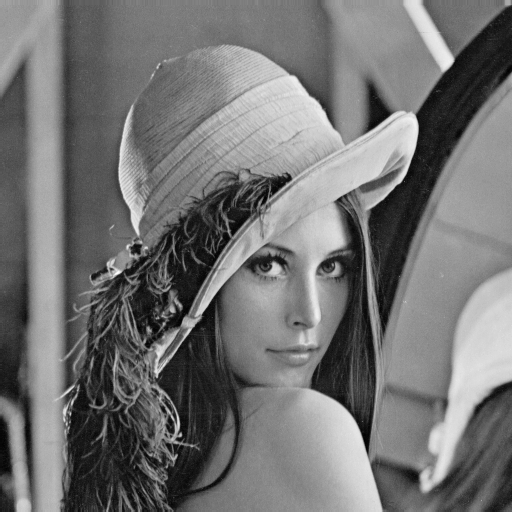
\includegraphics[width=\linewidth]{rev_image}
			%			\caption{Input images B1}
			%		\end{figure}
			&
			%		\begin{figure}
			%			\centering
			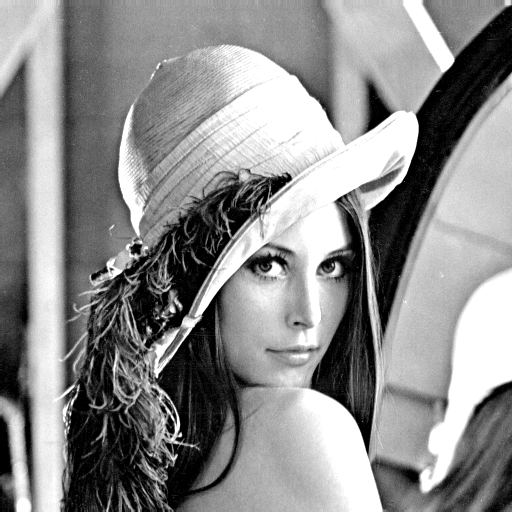
\includegraphics[width=\linewidth]{normalized_lena}
			%			\caption{Input images B1}
			%		\end{figure}
			\\
			\textit{Original} Lena Söderberg (1972) &
			\textit{Normalized}
		\end{tabular}
		
		The source code for the 
		
		\begin{tabular}{@{}p{.45\linewidth}@{\hspace*{.1\linewidth}}p{.45\linewidth}@{}}
			%		\begin{figure}
			%			\centering
			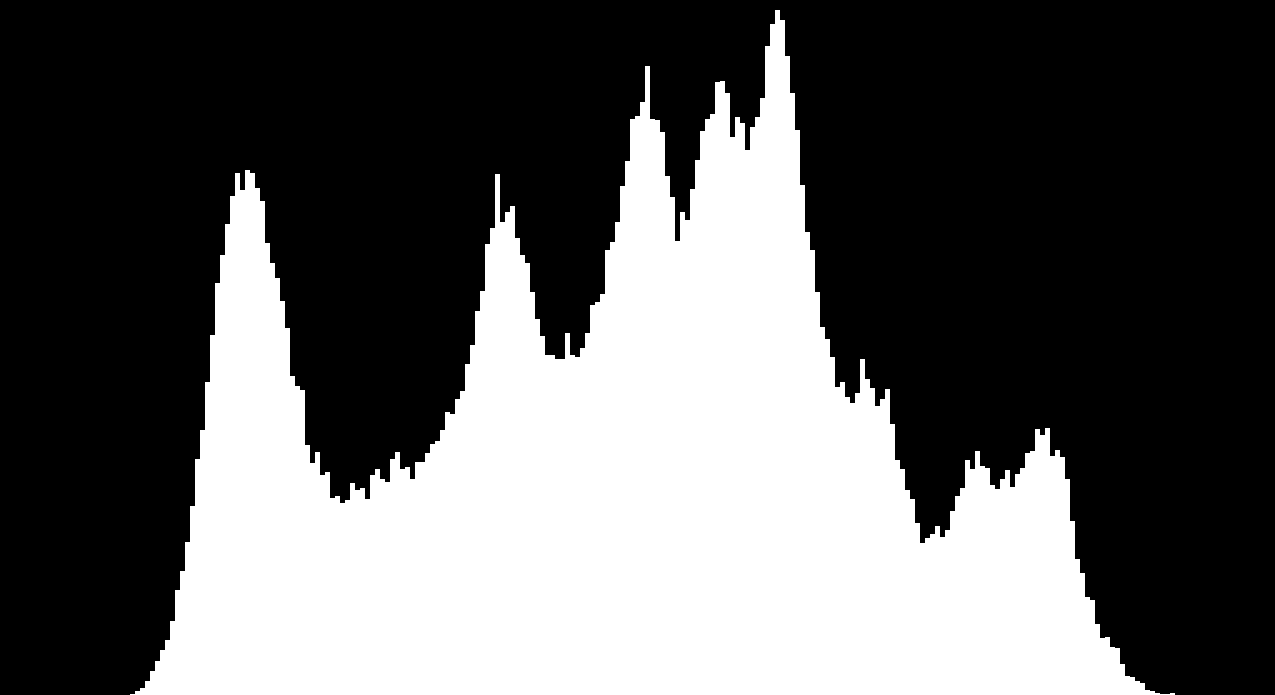
\includegraphics[width=\linewidth]{histogram_lena}
			%			\caption{Input images B1}
			%		\end{figure}
			&
			%		\begin{figure}
			%			\centering
			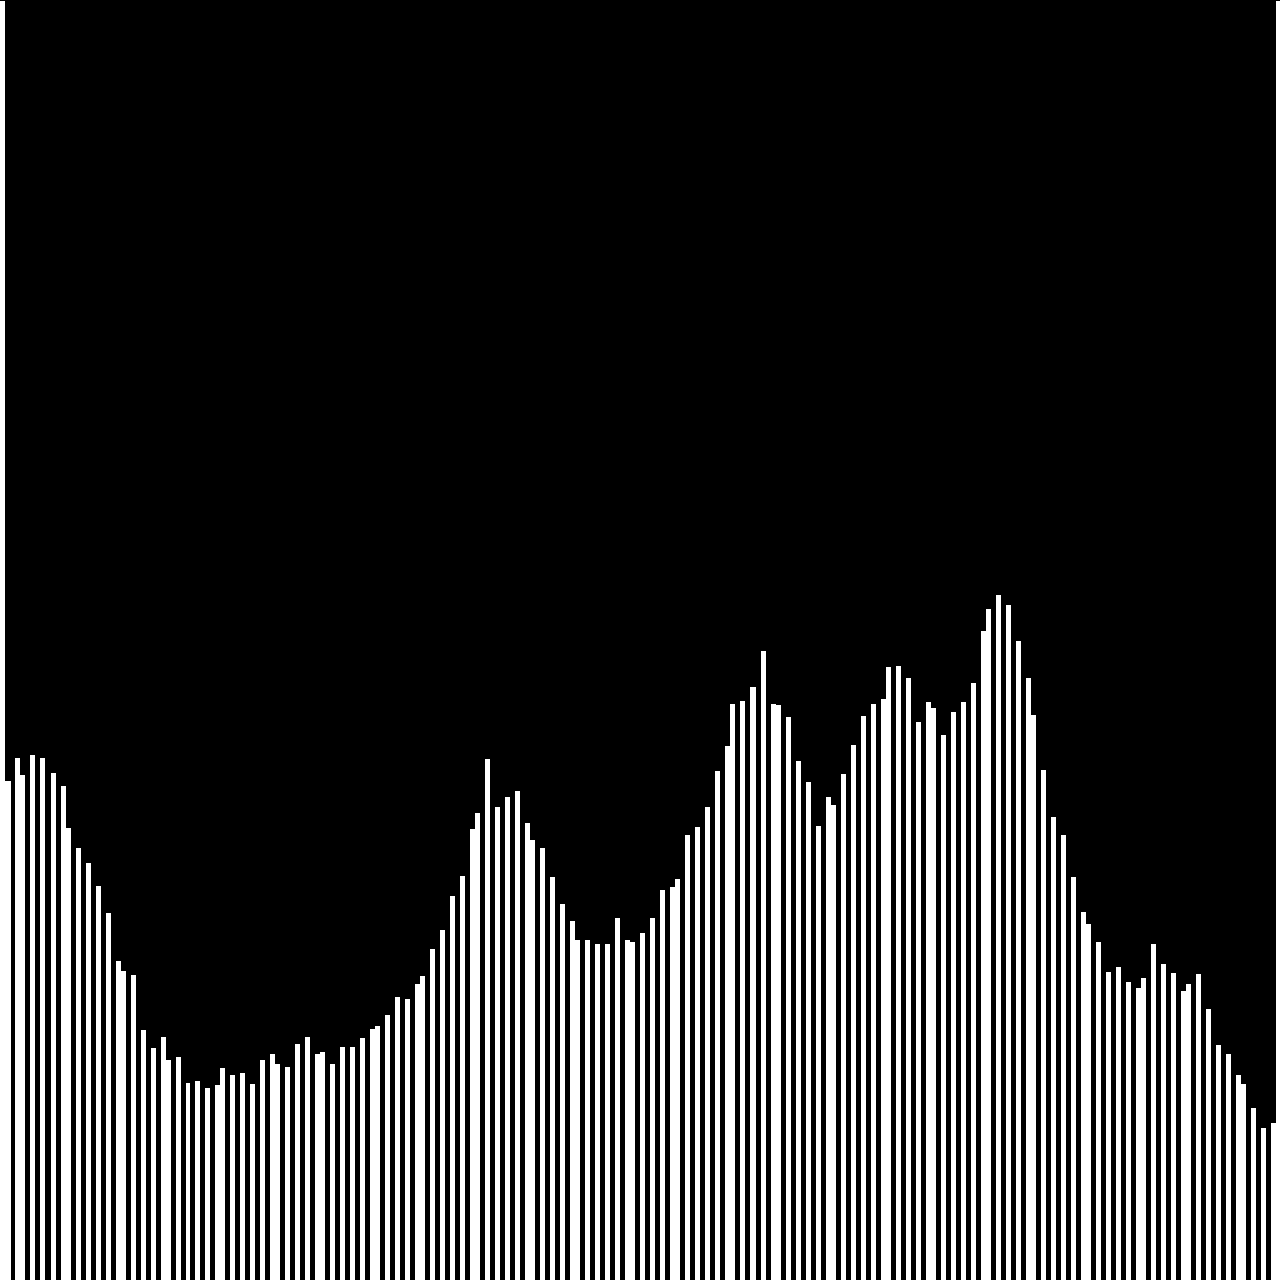
\includegraphics[width=\linewidth]{histogram_normalized_lena}
			%			\caption{Input images B1}
			%		\end{figure}
			\\
			\textit{Histogram of original} Lena Söderberg (1972) &
			\textit{Histogram of normalized image, values are linearly shifted}
		\end{tabular}
	\subsection{Fourier-Transform}
	
	You can simply combine two one-dimensional Discrete Fourier-Transform (DFT) functions with each other to obtain a two-dimensional one.

	With the following 1D DFT:
	
	\begin{align*}
		\hat{a}_{k} &= \sum\limits_{m = 0}^{M - 1} a_m \cdot e^{-2 \pi i \frac{mk}{M}} \\
	\end{align*}
	
	We can then follow the 2D DFT as follows:
	
	\begin{align*}
	&\sum\limits_{m = 0}^{M - 1} \hat{a}_{ml} \cdot e^{-2 \pi i \frac{mk}{M}} \\
	=&\sum\limits_{m = 0}^{M - 1} \Big[ \sum\limits_{n = 0}^{N - 1} a_{mn} \cdot e^{-2 \pi i \frac{nl}{N}} \Big] e^{-2 \pi i \frac{mk}{M}} \\
	=& \sum\limits_{m = 0}^{M - 1} \sum\limits_{n = 0}^{N - 1} a_{mn} \cdot e^{-2 \pi i \frac{mk}{M}} \cdot e^{-2 \pi i \frac{nl}{N}} \\
	=& \hat{a}_{kl}
	\end{align*}
\end{document}
